\providecommand{\main}{../../../..}
\documentclass[\main/dresen_thesis.tex]{subfiles}
\begin{document}
  \label{sec:doubleLayers:pnr}
  
  \begin{figure}[tb]
    \centering
    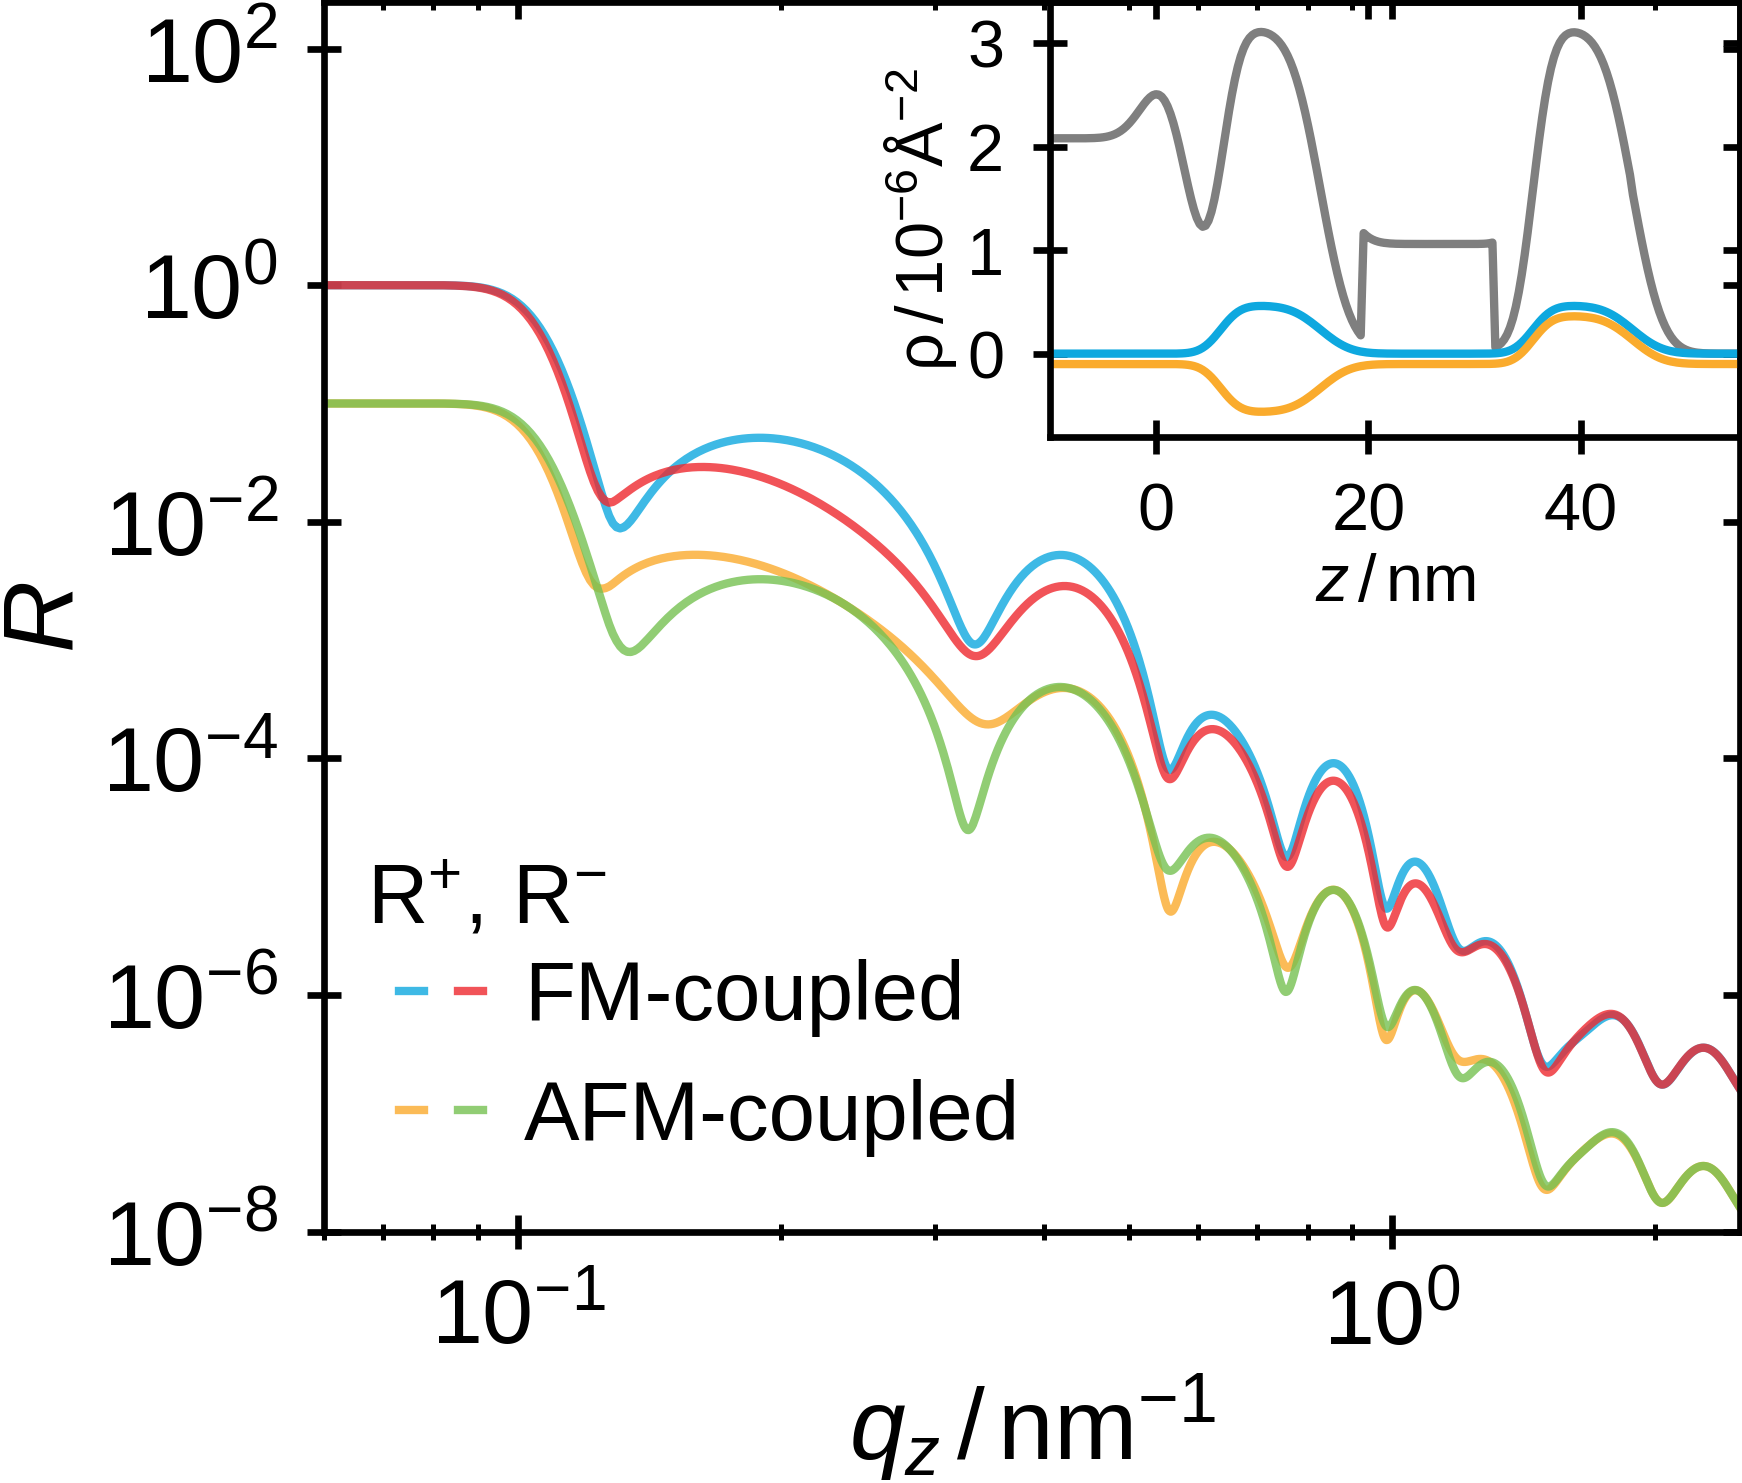
\includegraphics{doubleLayers_NR_simPNRsmallGap}
    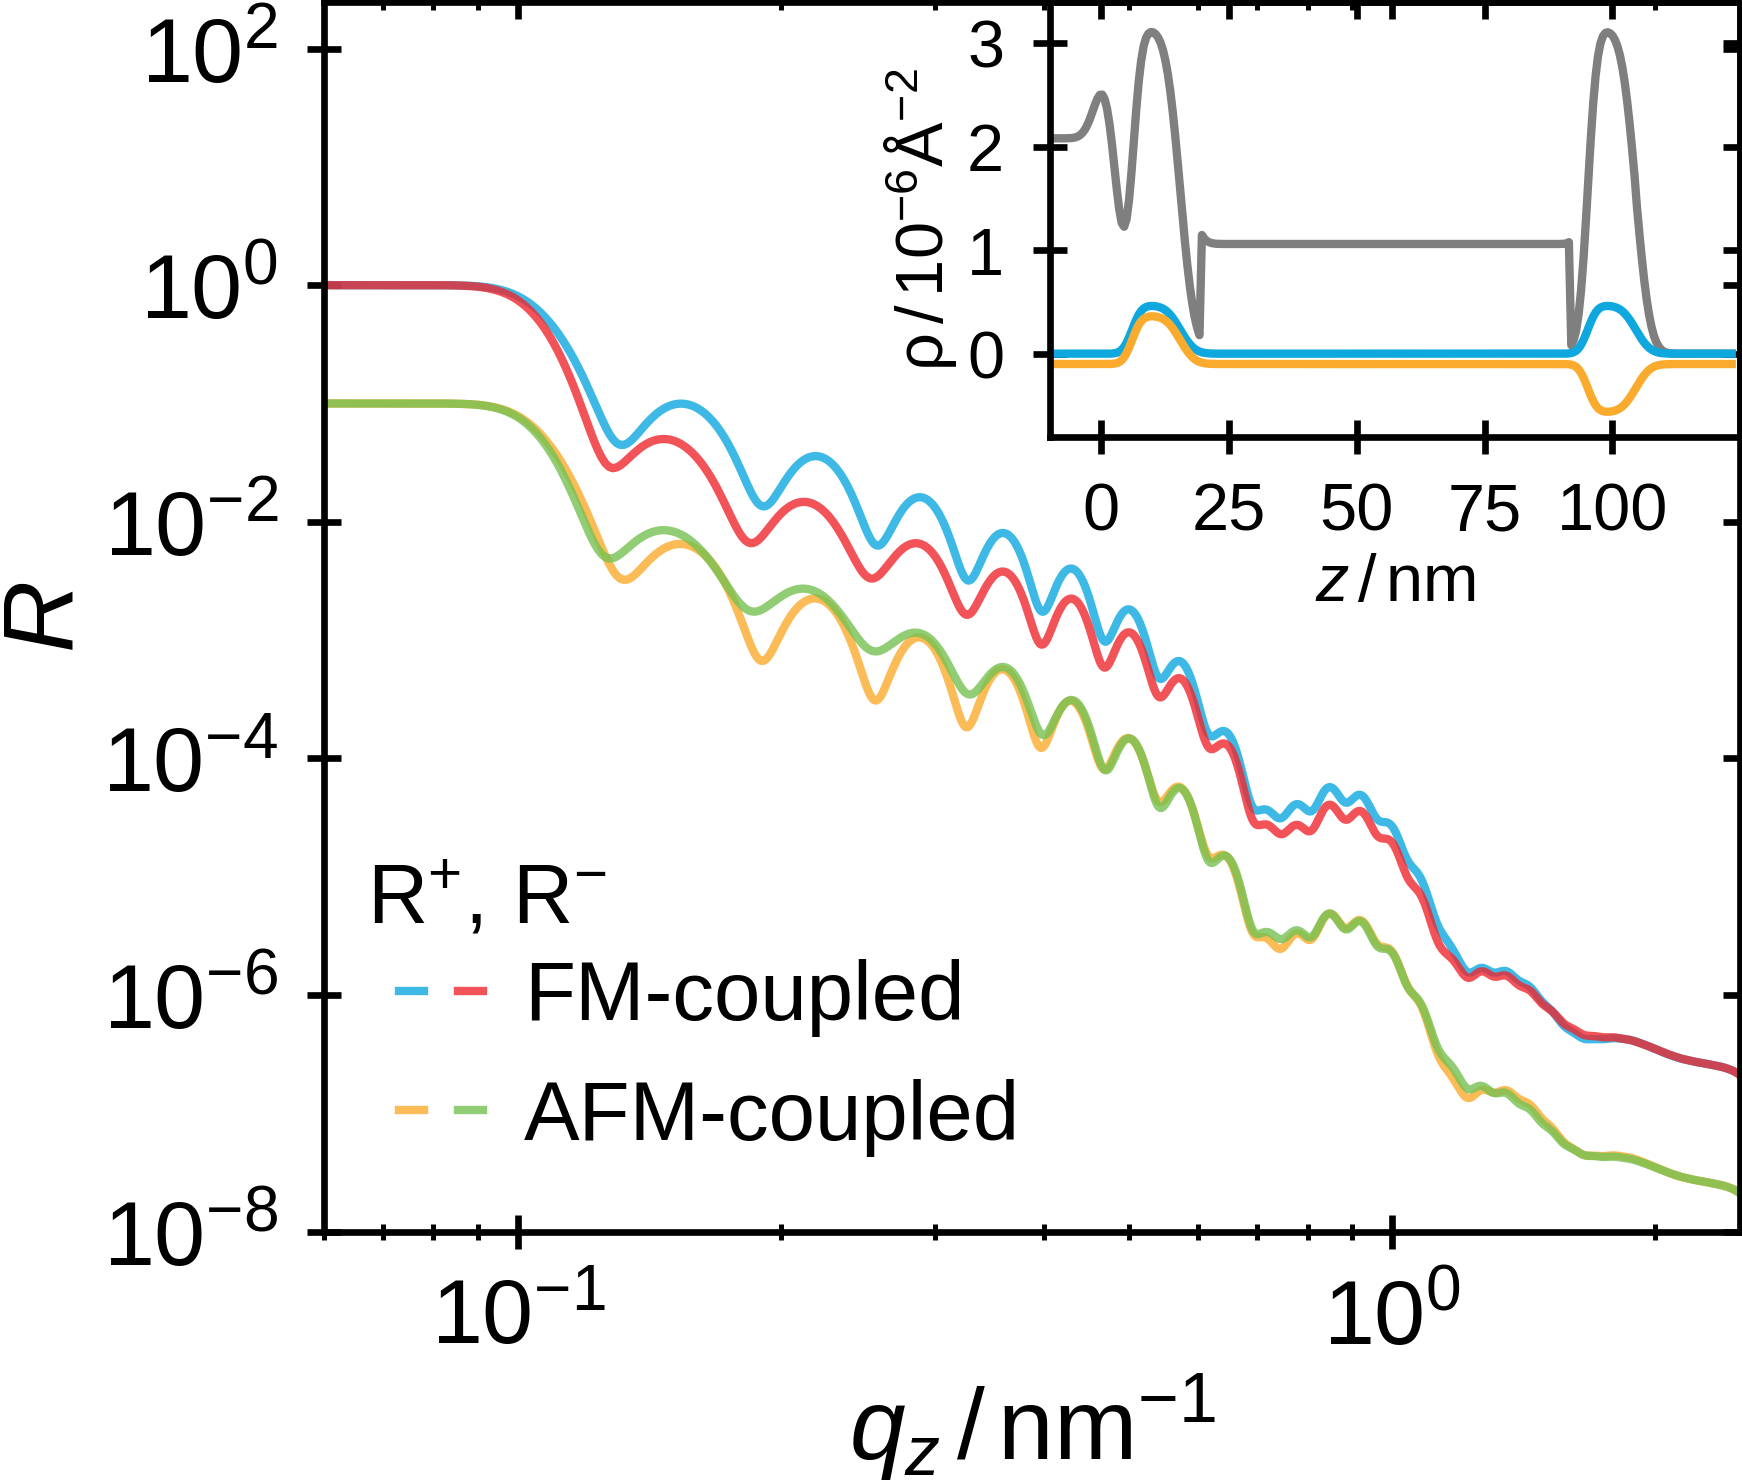
\includegraphics{doubleLayers_NR_simPNR}
    \caption{\label{fig:doubleLayers:pnrSimulation}Simulation of the half-polarized neutron reflectivities of double layers with the properties determined by the monolayer fit in \refsec{sec:monolayers:structure:verticalModel}. Shown is the expected splitting of a sample where both magnetic layers point in the same direction and where they are antiparallel once for a sample with a PMMA layer of small thickness (left) and large thickness (right).}
  \end{figure}

  Using polarized neutron reflectometry, the magnetic profile of the double layers is studied with depth resolution.
  With the result of the monolayer fit in \refsec{sec:monolayers:structure:verticalModel}, the expected reflectivity for $R^{+}$ and $R^{-}$ is simulated in \reffig{fig:doubleLayers:pnrSimulation} to discuss the basic differences that can be expected from the experiment.
  If the two layers are magnetized in parallel, as expected at a saturating magnetic field, a homogeneous splitting of the two channels is observed, where a clear separation between the maxima in $R^{+}$ and $R^{-}$ is visible.
  For the case, where the two layers are aligned antiparallel, the splitting reduces and in the case of  either a small or large PMMA gap, the maxima in the Kiessig fringes are touching one another and the splitting is only found in between.
  For the larger PMMA thickness sample, the splitting is visible from the critical edge up to the correlation peak around $0.9 \unit{nm^{-1}}$ that corresponds to the length scale of the single layers in the equally aligned case.
  Whereas for the antiparallel aligned case, around the critical edge and the correlation peak, both channels overlap and only a splitting in the intermediate $q$ - range of the Kiessig fringes is visible.
  Close inspection also shows that the splitting might invert as to which of the two channels $R^{+}$ and $R^{-}$ has the higher reflectivity as the simulations shows for the larger gap sample with $R^{-} > R^{+}$, whereas the simulation of the smaller gap is showing $R^{-} < R^{+}$.
  This is dependent on whether it is chosen that the upper layer is antiparallel to the beam polarization or whether the lower layer is, as the other choice results in the same reflectivities but with the behaviour of the two channels $R^{+}$ and $ R^{-}$ interchanged.
  \\

  \begin{figure}[tb]
    \centering
    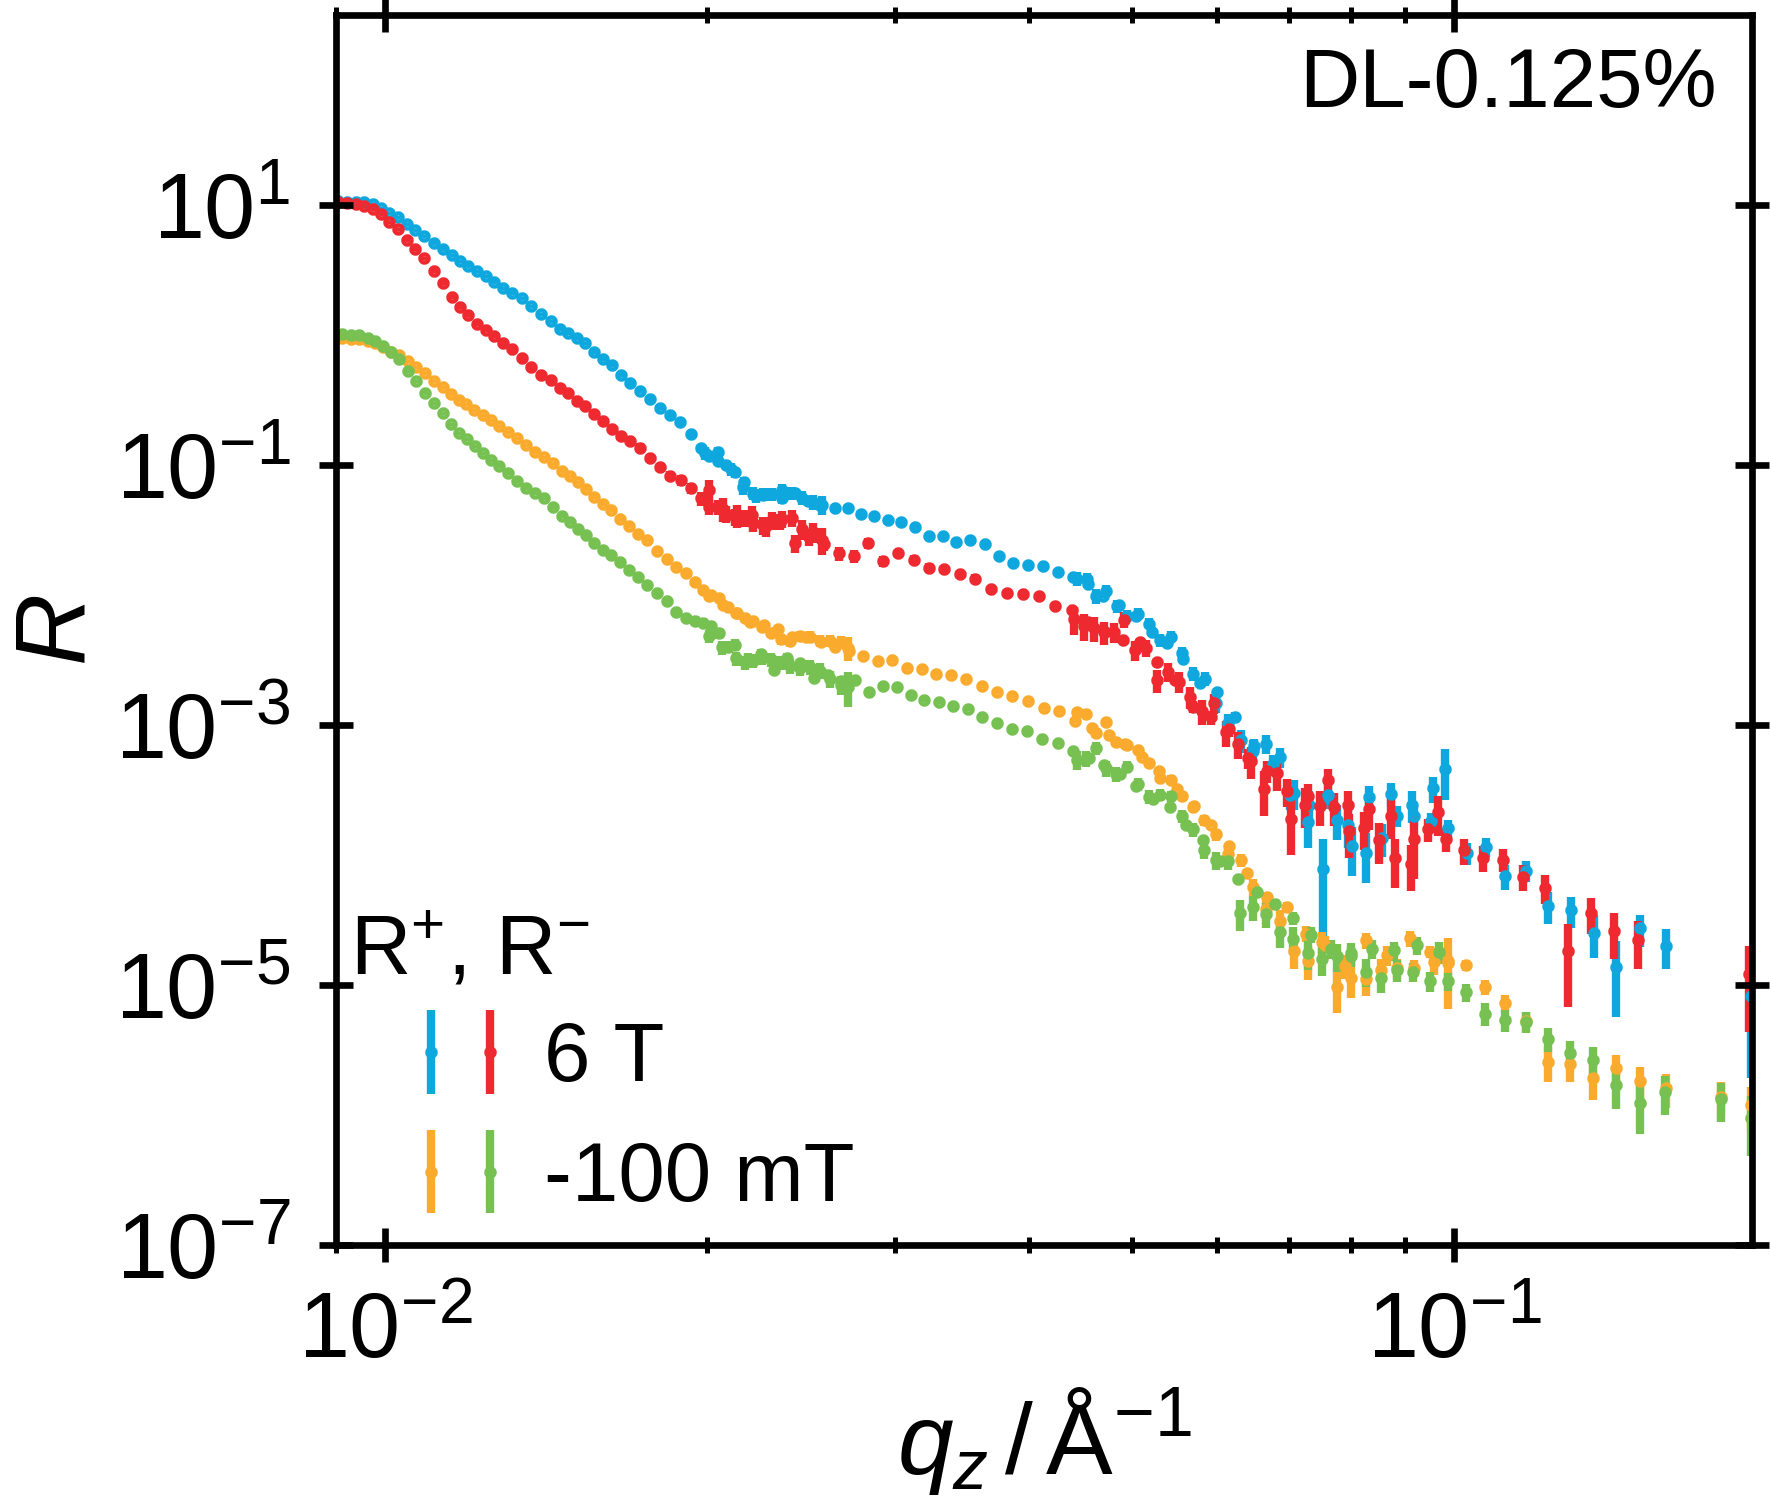
\includegraphics{doubleLayers_VerticalStructure_DL-0-125_PNR_ZFC5K}
    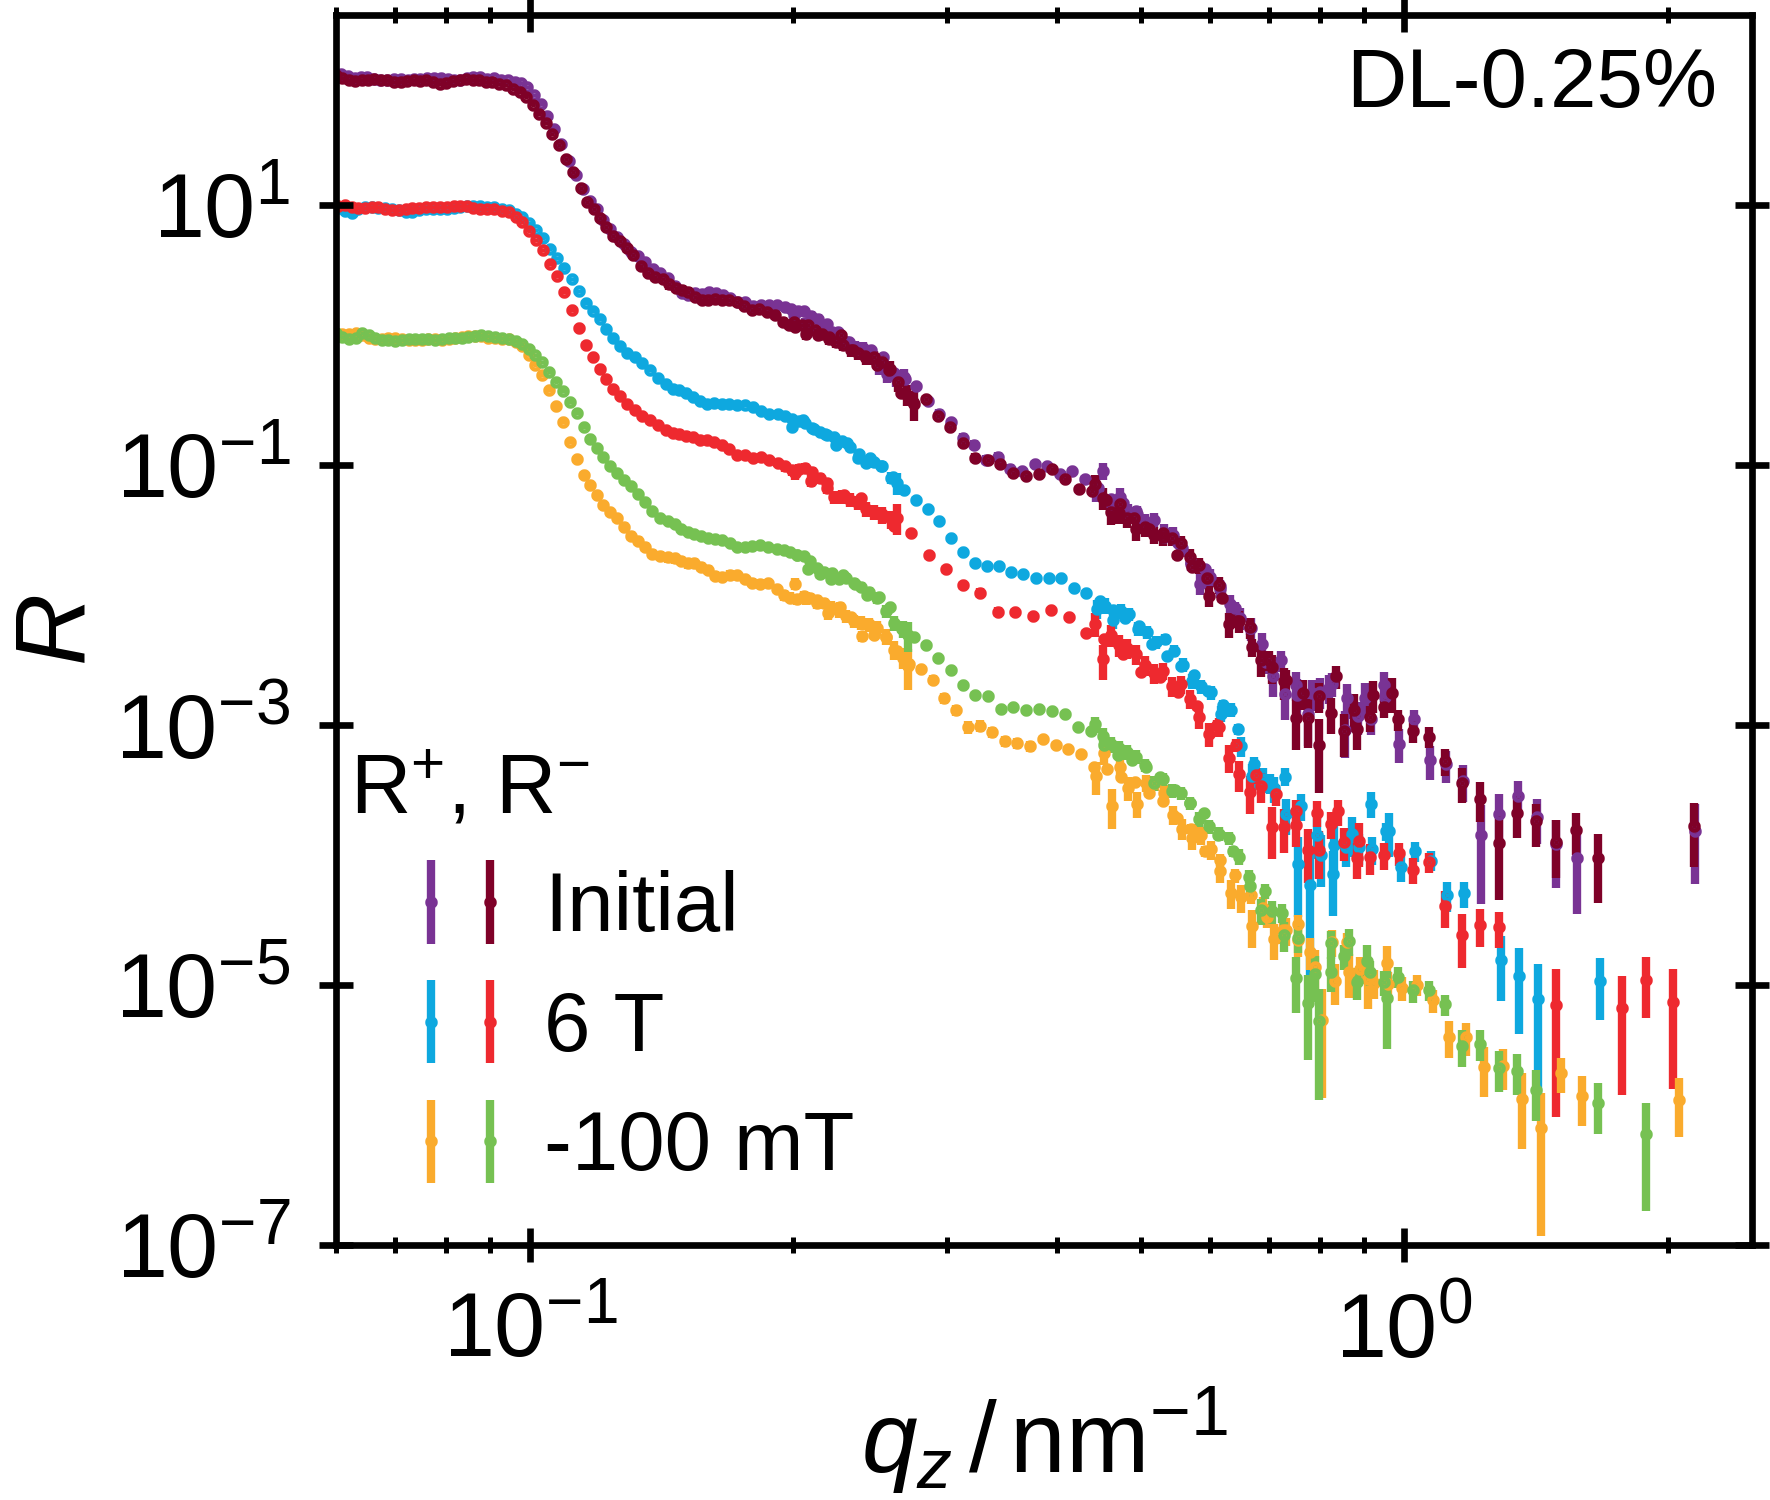
\includegraphics{doubleLayers_VerticalStructure_DL-0-25_PNR_ZFC5K}
    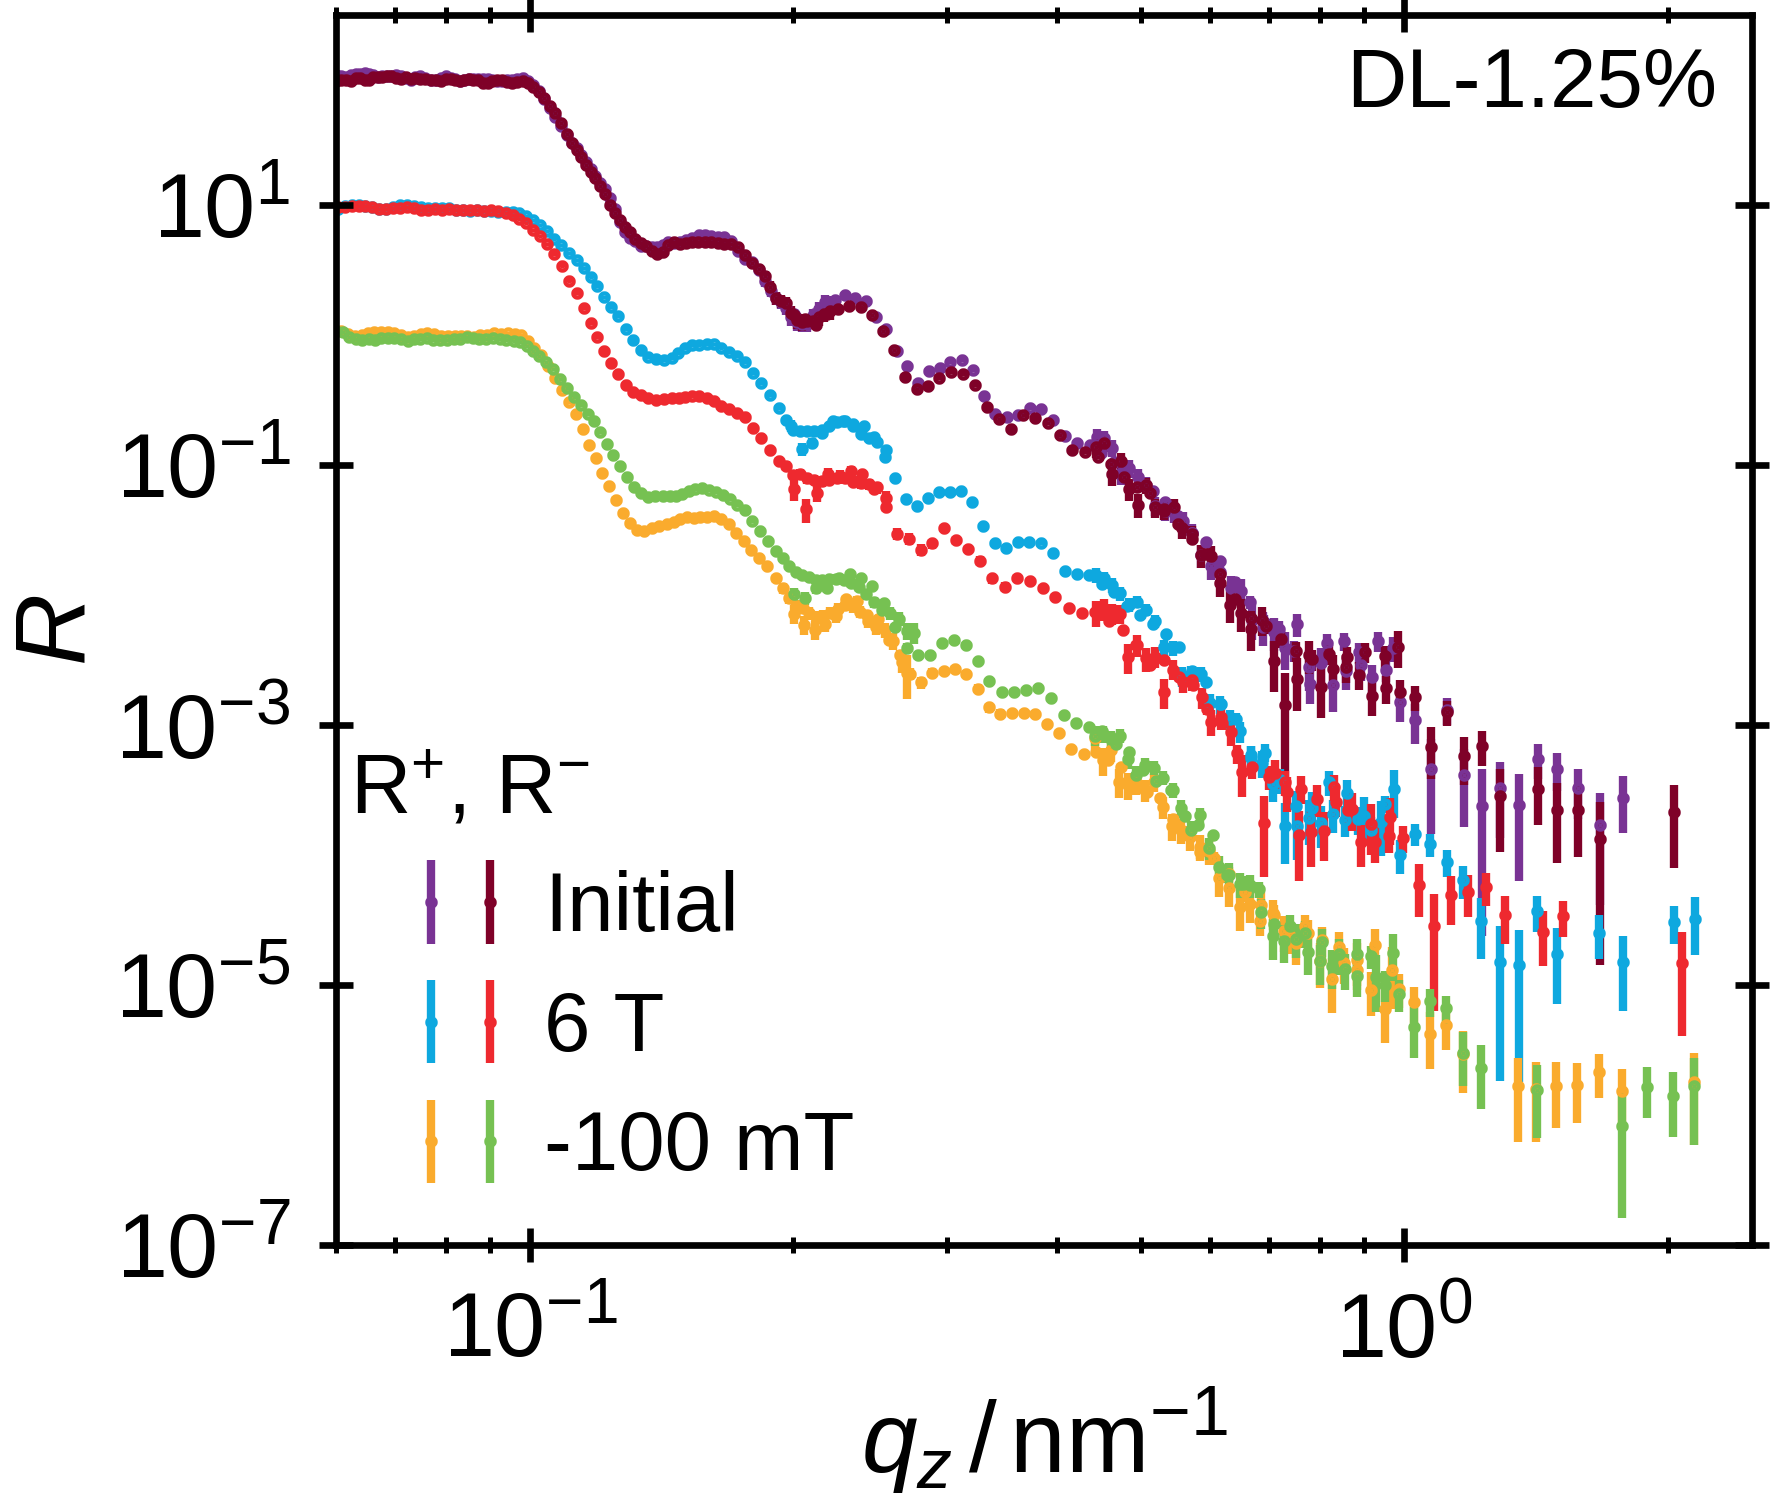
\includegraphics{doubleLayers_VerticalStructure_DL-1-25_PNR_ZFC5K}
    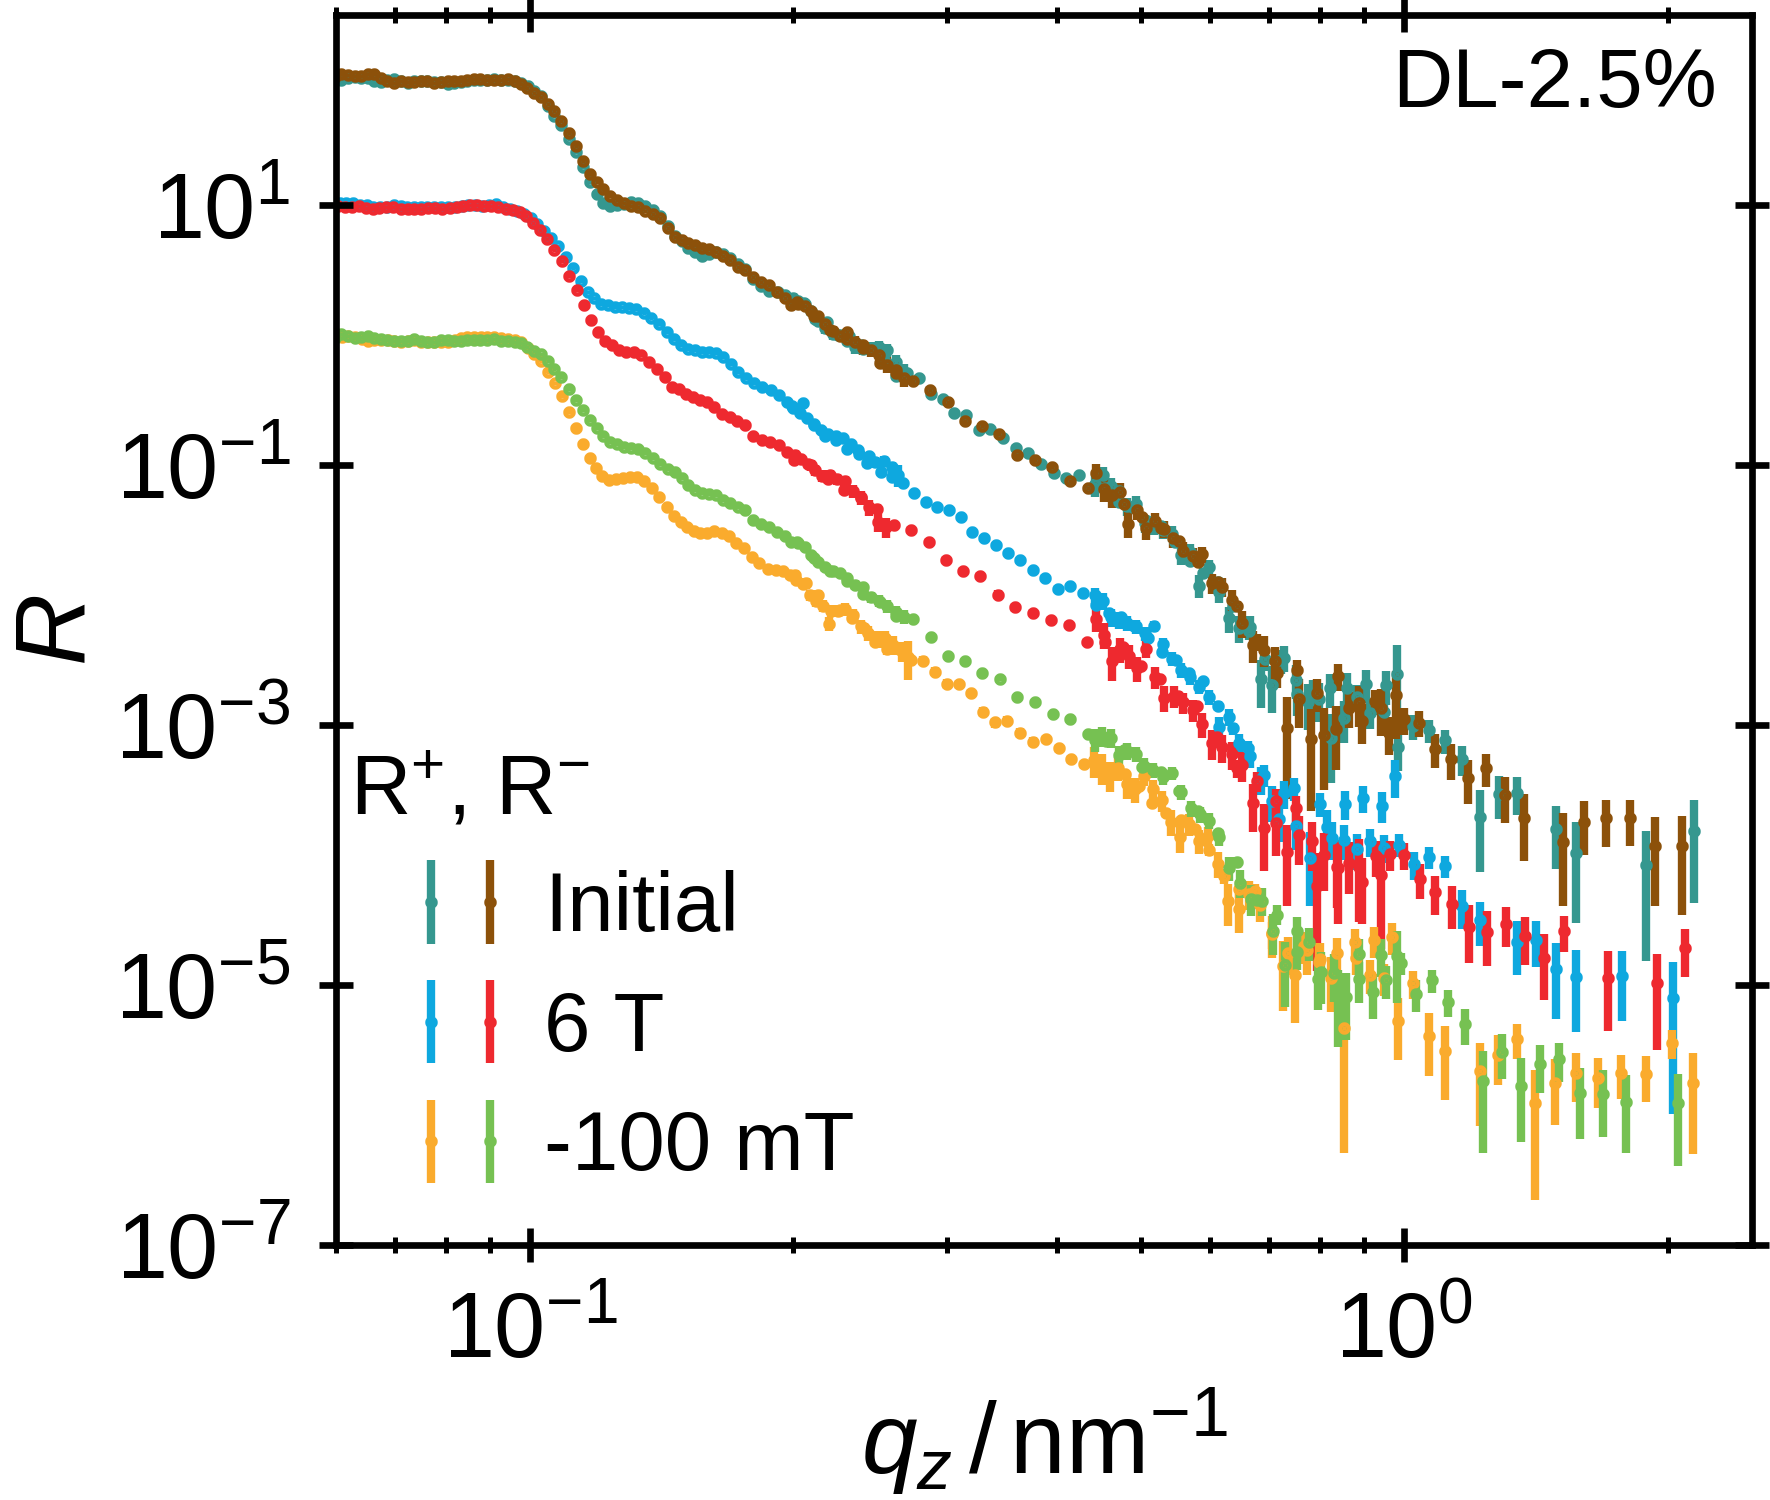
\includegraphics{doubleLayers_VerticalStructure_DL-2-5_PNR_ZFC5K}
    \caption{\label{fig:doubleLayers:pnrData}Polarized neutron reflectometry of DL-0.125\%, DL-0.25\%, DL-1.25\% and DL-2.5\% measured at $5 \unit{K}$ after zero-field cooling. For all samples but DL-0.125\%, the reflectivity at guide field after cooling is shown and furthermore for all samples, measurements at a field of $6 \unit{T}$ and subsequently $-100 \unit{mT}$ are displayed.}
  \end{figure}
  Using the discussed model, the reflectivity of the double layers shown in \reffig{fig:doubleLayers:pnrData} are analyzed.
  In all cases a homogeneous splitting is observed at $6 \unit{T}$, with a clear separation of $R^{+}$ and $R^{-}$ as it would be expected for a homogeneously magnetized sample.
  For the study of the ground state and dipolar interaction, the interesting cases are the measurements directly after zero-field cooling and in remanence after application of a saturating field.
  The samples DL-0.25\%, DL-1.25\% and DL-2.5\% show that initially after zero-field cooling no strong splitting is visible.
  Slight differences in $R^{+}$ and $R^{-}$ are however visible in both DL-1.25\% and DL-2.5\%.
  The observations indicate that macroscopically the sample is in a magnetically disordered state with no preference of the in-plane magnetization in direction of the applied field versus the direction antiparallel to it.
  In the remanent state, a clear separation of the two states at the peaks of the Kiessig fringes is visible.
  Using the result of the previously discussed simulation, this observation can be used to exclude an antiferromagnetic alignment in each case.
  This is in agreement with the macroscopic magnetization measurement in \refsec{sec:doubleLayers:vsm}, where an antiparallel alignment of the layers at low fields would otherwise become visible by a strong decrease in the magnetization magnitude instead of the observed wide hysteresis in each case.

  What however can not be excluded from the qualitative discussion of the data is an only partially antiparallel alignment of the layers due to interlayer dipolar coupling combined with a partially ferromagnetic alignment.
  To discuss this, a detailed quantitative evaluation by scattering length density profile models is necessary.
\end{document}